\documentclass[10pt,a4paper]{article}
\usepackage[utf8]{inputenc}
\usepackage[spanish]{babel}
\usepackage{amsmath}
\usepackage{amsfonts}
\usepackage{amssymb}
\usepackage{graphicx}
\usepackage{float}
\usepackage{multicol}
\usepackage{subcaption}
\usepackage{cite} % para contraer referencias
\usepackage[left=2.00cm, right=2.00cm, top=2.00cm, bottom=2.00cm]{geometry}
\author{UTP student}
\title{determinación de la gravedad}
\begin{document}
	\begin{figure}[H]
		\raggedright
		
\includegraphics[scale=0.1]{imagenes-proyecto/logo_utp.png}
	\end{figure}

%\begin{center}
%	\rule{170mm}{0.4mm}
%\end{center}

	\begin{center}
		{\huge \textbf{DETERMINACIÓN EXPERIMENTAL DE LA ACELERACIÓN DE LA GRAVEDAD UTILIZANDO UN PÉNDULO SIMPLE}} \\
		
		\vspace{2mm}
		\Large {1er Jhanmer Paucar $^{1}$, 2do Cristell Sandoval $^{2}$, 3er Nilson Martin$^{3}$}
		
		\vspace{6mm}
		$^{1}$ \textit {Universidad Tecnológica del Perú. Ingeniería de Sistemas e Informática - sede Lima sur.} 
		$^{2}$ \textit {Universidad Tecnológica del Perú. Ingeniería de Sistemas e informática - sede Lima norte.} 
		$^{3}$ \textit {Universidad Tecnológica del Perú. Ingeniería Industrial - sede Lima sur.} 
	\end{center}
    \begin{center}
    	\rule{150mm}{0.2mm}
    \end{center}
%%%%%%%%%%%%%%%%%%%%%%%%%%%%%%%%%%%%%%
%%%%%%%%%%%%%%%%%%%%%%%%%%%%%%%%%%%%%%
% Resumen
\begin{abstract}
	
Este presente trabajo de investigación se determina de manera experimental el módulo de la aceleración de la gravedad utilizando un péndulo simple y unos materiales básicos y comunes que tenemos en casa. Para esto usamos el cronómetro para medir el tiempo del número de oscilaciones que dará nuestra masa puntal. El valor del periodo se calcula a partir de los promedios de los tiempos de oscilaciones, así mismo de las diferentes longitudes de una cuerda de nilón en la que se sujeta la masa puntual. Con estas medidas, se analiza la relación entre el periodo del péndulo y la longitud. Luego haber graficado nuestra tabla y realizado el ajuste lineal del periodo al cuadrado y la longitud del péndulo se obtiene una pendiente y el punto de corte o intercepto, en la que existe una relación lineal entre el periodo y la longitud del péndulo, ya que al linealizar la recta pasa al punto de origen y el punto de corte es insignificante y nuestro factor de correlación se acerca a 1, y con estos estos datos ya podemos determinar el valor de la gravedad experimental. Entonces, teniendo la gravedad experimental se observa que no es el valor de referencia de gravedad de la tierra, pero el error porcentual que se cálculo es $(3\%)$ y esto se debe a toma de datos en del experimento, ya sea por la resistencia del aire en el que se desarrolló el experimento o las tomas de tiempos de los números de oscilaciones calculadas por el cronómetro.. Así mismo se realizó otro experimento para determinar si existe una relación lineal entre el Periodo y la masa, pero se concluyó que no existe tal relación, ya que la pendiente es casi 0 es decir insignificante también el factor de correlación es muy pequeña. 

\end{abstract}

\begin{center}
	\rule{150mm}{0.2mm}
\end{center}
%%%%%%%%%%%%%%%%%%%%%%%%%%%%%%%%%%%%%%
\vspace{2mm}
\underline{\textbf{Palabras clave:}} \hspace{1mm} \textit{Péndulo simple, gravedad, ajuste lineal, oscilaciones, incertidumbre, propagación de incertidumbres, resistencia del aire, relación lineal.}
\vspace{4mm}

%%%%%%%%%%%%%%%%%%%%%%%%%%%%%%%%%%%%%%
%%%%%%%%%%%%%%%%%%%%%%%%%%%%%%%%%%%%%%
% 	Introducción
\begin{multicols}{2}
	\section{Introducción}
En estos tiempos de Covid-19, la educación ha tenido diferentes problemas para poder continuar con su labor, es por ello que se buscó diferentes formas para que los educadores lleguen a los alumnos y así se permita que fluya la enseñanza en la ciencia por el medio del uso de herramientas digitales y sea accesible para que beneficien las investigaciones del manejo de situaciones problemáticas experimentales de la física. Este proyecto fue iniciado ya hace muchos años por el famoso científico Galileo Galilei \cite{cespedesprimer}, quien estableció el principio del péndulo.\\
El presente trabajo tiene como objetivo determinar experimentalmente el valor de la aceleración de la gravedad por medio del péndulo simple, empezando de la relación que existe entre el cuadrado del periodo del péndulo y la longitud del péndulo, puesto que estos parámetros muestran dependencia lineal. Este trabajo apoya mucho a los estudiantes de primeros años de ingeniería en esta época de pandemia, ya que se puede realizar con herramientas que encontramos en casa y con el apoyo del tutor en línea. Podrán observar como con una maqueta muy simple se puede encontrar este módulo de la aceleración. Pese a esta situación mundial el no a ver estado de forma presencial en la universidad, no afecto mucho puesto que ayudo a romper el tabú que solo en un laboratorio se puede hacer ciencia.

%%%%%%%%%%%%%5%%%%%%%%%%%%%%%%%%%%%%%%%%%%%
%%%%%%%%%%%%%%%%%%%%%%%%%%%%%%%%%%%%%%%%%%%
% Marco teórico
\section{Marco teórico}

Para determinar el módulo de aceleración de la gravedad se puede determinar a través de distintos métodos como un péndulo simple, caída libre e instrumentos de medición. Para este experimento usaremos el método de Péndulo simple, que según \cite{sears1986fisica} consiste en tener una masa puntual suspendida sobre una cuerda de masa despreciable y sin estirarse o deformarse, de tal forma que la masa oscilará no de forma recta sino en una trayectoria de arco circular, de modo que el radio será la longitud del péndulo $(l)$. Por otro lado, las dimensiones de la cuerda deben ser 10 a 15 veces mayor a las dimensiones de la masa.\\\vspace{1mm}

En la Figura 1, se visualiza las fuerzas que actúan sobre la masas, es decir se observa el DCL, \cite{tecalco2021aproximacion} acorde con la segunda ley de Newton de movimiento en la dirección tangencial, se concluye que la sumatoria de fuerza $F_{t}$ debe ser igual a la masa $(m)$ por aceleración tangencial$(a_{t})$.

\begin{equation}
	\sum F_{t}= m a_{t}
	\label{1}
\end{equation}
Luego, observamos que la fuerza de gravedad no está en equilibrio, por lo que descomponemos las fuerzas tanto en el eje tangencial y el eje radial, entonces para la fuerza que actúa sobre la dirección tangencial es el peso, y como vemos que esa componente del peso va en dirección contraria, vendría hacer negativo $(-)$.
% sumatorias de fuerzas igual m por a luego simplificamos y hallaremos la siguiente ecuación hacer ma';ana
\begin{equation}
	-mg \sin \theta = ma
	\label{2}
\end{equation}
\begin{equation}
	a = -g \sin \theta
	\label{3}
\end{equation}
Entonces, vemos que la aceleración es $(-g \sin \theta)$, pero recordemos que la aceleración es la segunda derivada de la posición  \cite{rendon2021sistema}, pero como se observa la gráfica \ref{ima-DCL} la masa puntal realiza una trayectoria de un arco, así que sería la segunda derivada de $(s)$ como se observa en la ecuación \ref{4}.
\begin{equation}
	F_{t}= -mg \sin \theta = \frac{\mathrm{d}^2s }{\mathrm{d} t^2}
	\label{4}
\end{equation}
Además, vemos que $(s)$ es la posición de la masa, y vemos que se cumple el famoso $L= \theta R$, pero el radio vendría hacer la longitud de la cuerda y así mismo $L$ por s, por lo tanto, quedaría como $s = \theta L $, y observamos que la ecuación quedaría reducida de esta manera.
\begin{equation}
	\frac{\mathrm{d^{2}\theta} }{\mathrm{d} t^{2}}=\frac{-g}{L}\sin \theta
	\label{5}
\end{equation}

Vemos que la ecuación \ref{5} no es un MAS, entonces para que se asemeje a un armónico simple, decimos que $\sin \theta$ sea $\theta$. En el caso de que el ángulo sea pequeño $ \theta \leq 10^{\circ{}}$, se cumple que $ \theta \approx \sin \theta $, y considerando la segunda ley de Newton, la ecuación \ref{4} se puede escribir como:


\begin{equation}
	\frac{\mathrm{d^{2}\theta} }{\mathrm{d} t^{2}}=\frac{-g}{L}\theta
	\label{7}
\end{equation}
Tomando en cuenta la ecuación \ref{7}; se obtiene frecuencia angular es: 
\begin{equation}
	\omega = \sqrt{\frac{L}{g}}
	\label{8}
\end{equation}
Pero sabemos que el periodo de un péndulo simple se halla de esta manera:
\begin{equation}
	T = \frac{2\pi }{\omega }
	\label{9}
\end{equation}
Entonces la ecuación para hallar el periodo de un péndulo simple será:
\begin{equation}
	T = 2\pi\sqrt{\frac{L}{g}}
	\label{10}
\end{equation}
\begin{figure}[H]
	\centering
	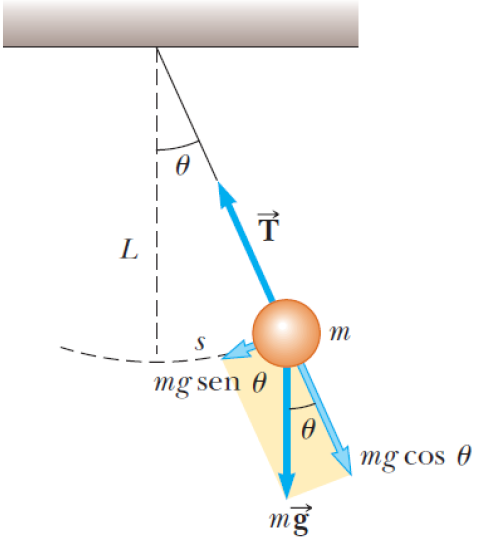
\includegraphics[scale=0.5]{imagenes-proyecto/imagen_pendulo.png}
	\captionsetup{justification=centering}
	\caption{Diagrama de cuerpo libre para un péndulo simple.}
	\label{ima-DCL}
\end{figure}

De la figura \ref{ima-DCL}, se indica que la masa puntal se descompone, tanto en el eje tangencial como en el eje radial, y la componente tangencial podemos decir que es una fuerza restauradora, como consecuencia el ángulo va disminuyendo mientras transcurre las oscilaciones, es decir que la masa puntual se aproxima a su posición de equilibrio.\\
Así mismo, vemos que hay una fuerza Tensión $T$, pero esa fuerza no necesita descomponerse, puesto que está en equilibrio.


%%%%%%%%%%%%%%%%%%%%%%%%%%%%%%%%%%%%%%%%%%
%%%%%%%%%%%%%%%%%%%%%%%%%%%%%%%%%%%%%%%%%%
% Materiales y métodos
\section{Metodología} % Detalles experimentales
Para realizar el experimento de determinar la aceleración de la gravedad mediante un péndulo simple, se abordó dos experimentos, respecto al primer experimento la longitud de péndulo fue variando, pero la masa se mantuvo constante, se usaron cinco medidas distintas, en donde la incertidumbre de la cuerda es de $ \pm 0.0005m$. Así mismo, para el segundo experimento la longitud del péndulo se mantuvo constante y la masa fue variando, de igual forma se usaron cinco masas distintas y su incertidumbre de la masa es de $ \pm 0.001m$, y para así poder determinar si existe una relación entre el periodo y la masa. Por otro lado, se usó materiales como, una cinta métrica, una cuerda de nilón, silicona en barra, una balanza electrónica, un transportador y por último un cronómetro. \\

{\textbf {Diseño:}} Luego para construir la  maqueta se usó básicamente madera, se optó por colocar un base rectangular y su posicionó un palo de madera de forma vertical luego en la parte superior del palo de madera se colocó otro palo pero esta vez de forma horizontal. Así mimo. se ubicó un gancho metálico pequeño en la parte extrema del palo horizontal para así sujetar la cuerda de nilón, además se reforzó con silicona, así mismo en la altura de gancho se situó un transportador para así medir el ángulo en que va a oscilar nuestra masa.
\begin{figure}[H]
	\centering
	\includegraphics[scale=0.3]{imagenes-proyecto/diseño.jpeg}
	\caption{Maqueta de nuestro péndulo simple.}
	\label{maqueta}
\end{figure}
 {\textbf {Instrumentos:}} Luego de haber terminado la maqueta, se procedió a usar instrumentos como una balanza electrónica para pesar la masa, una cinta métrica para poder medir la longitud del péndulo y por último se usó un cronómetro para poder calcular el tiempo de las oscilaciones, para este experimento vamos a tomar en cuenta cinco oscilaciones. \\
\begin{figure}[H]
	\raggedright
	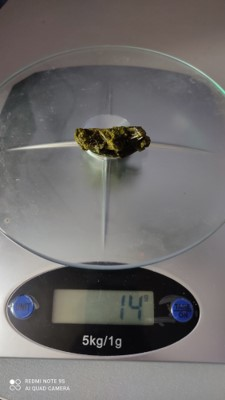
\includegraphics[scale=0.4]{imagenes-proyecto/instrumento1.jpg}
	\raggedleft
	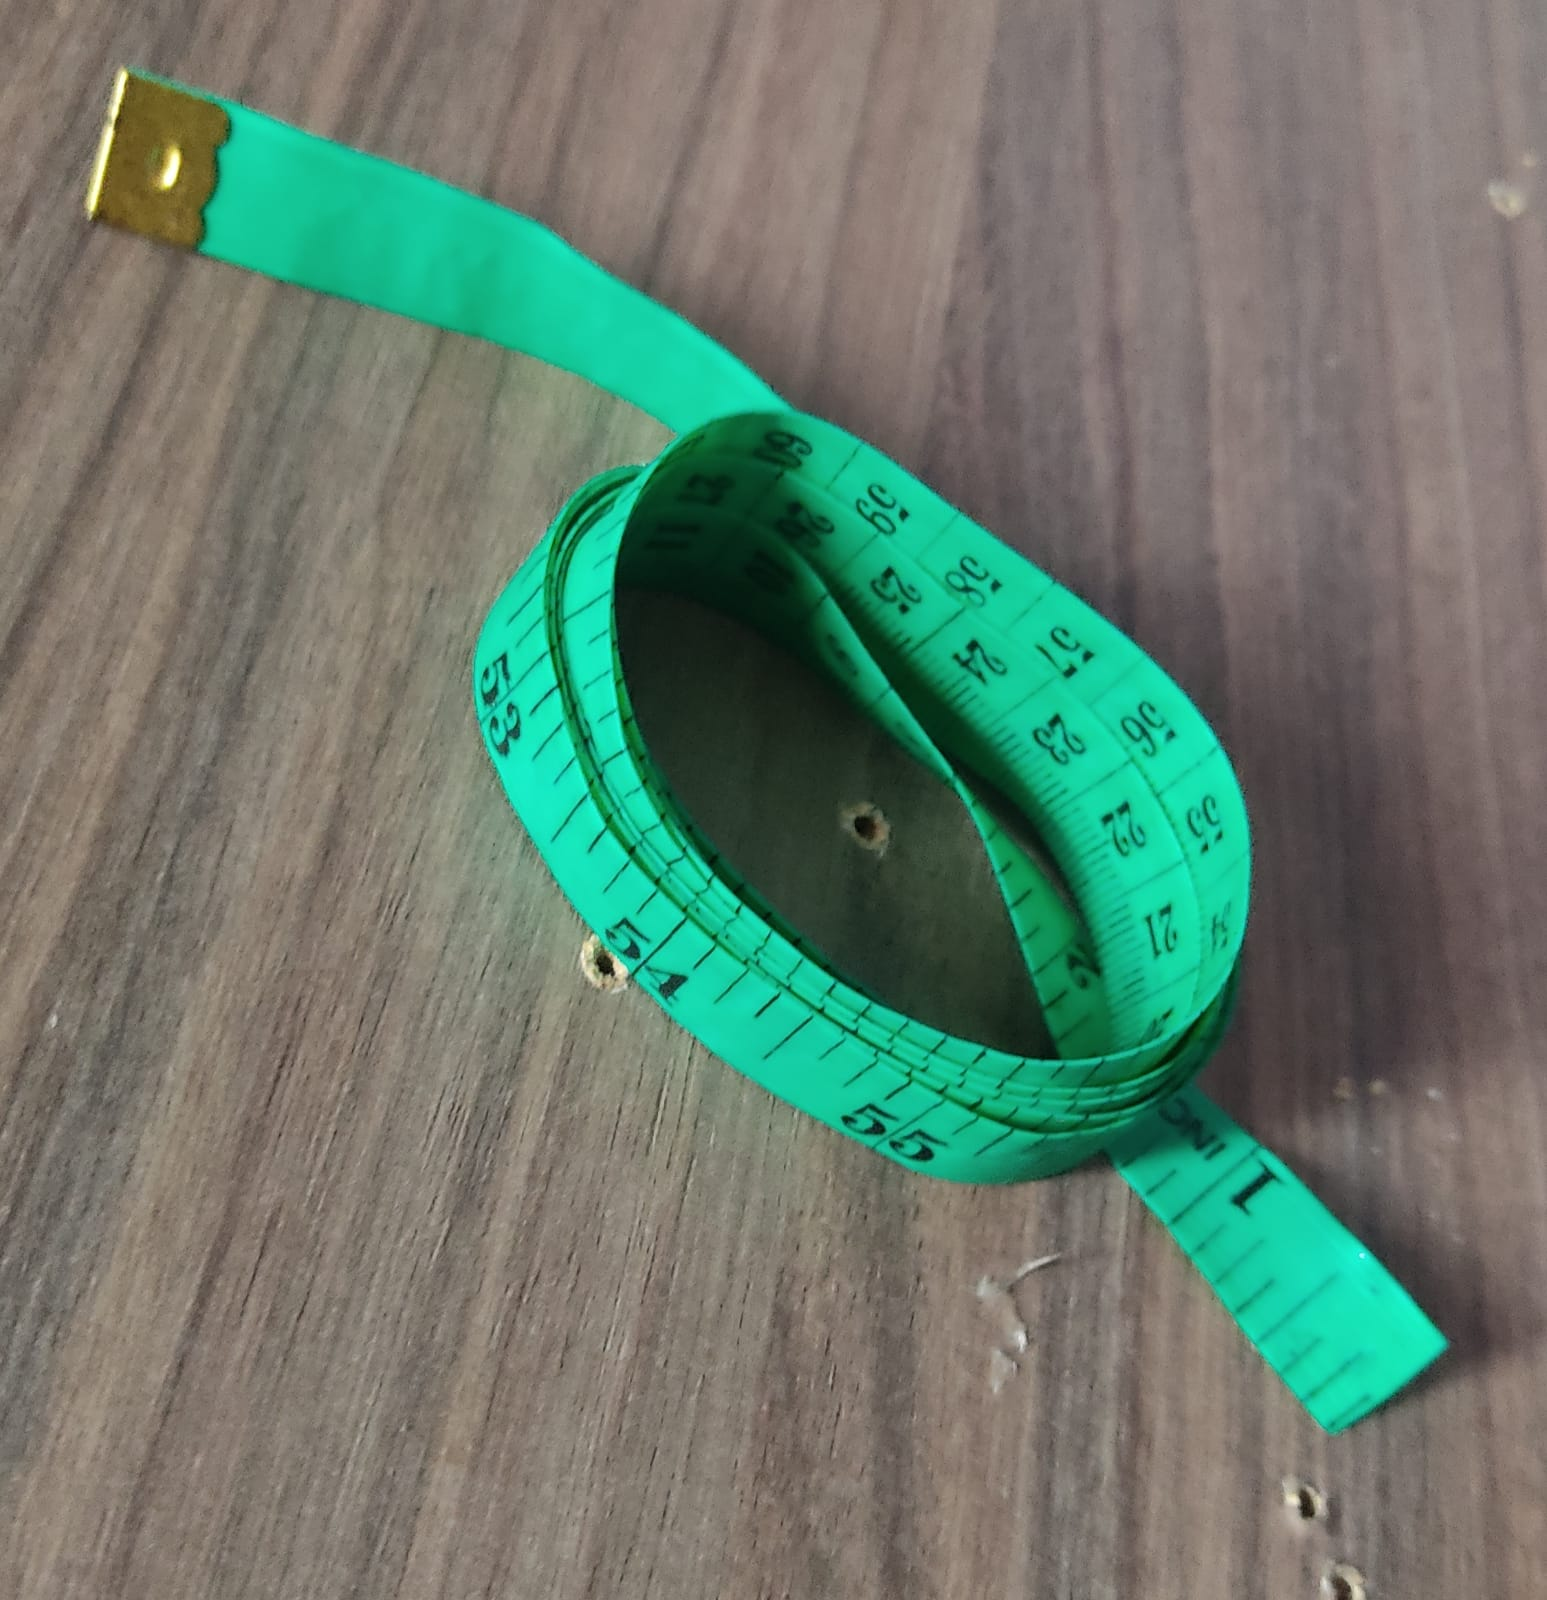
\includegraphics[scale=0.07]{imagenes-proyecto/cinta.jpeg}
	\captionsetup{justification=centering}
	\caption{Instrumentos para medir la longitud del péndulo y para pesar las masas.}
	\label{instrumentos}
\end{figure}
{\textbf {Equipos técnicos e informáticos:}}  Por otro lado, hemos optado por usar PETH como software de ayuda en la realización de nuestro experimento, puesto que nos aporta una expectativa clara de cómo se comporta un péndulo simple y también hemos usado MicrosoftExcel para poder graficar nuestros dos experimentos y realizando las configuraciones para saber el ajuste lineal.
\begin{figure}[H]
\raggedright

\includegraphics[scale=0.18]{imagenes-proyecto/phet.png}   

\raggedleft

\includegraphics[scale=0.03]{imagenes-proyecto/excel.png}
\captionsetup{justification=centering}
\caption{Programas informáticos para realizar gráficos y simuladores para comprender el péndulo.}
\label{programas}
\end{figure}
%%%%%%%%%%%%%%%%%%%%%%%%%%%%%
%Resultasos

\section{Resultados}
Con todas las muestras desarrolladas en la sección de metodología se obtuvo los siguientes resultados. Se procede a realizar el experimento teniendo en cuenta que el péndulo debe estar a cierto ángulo para que se cumpla el principio de un péndulo simple, en esta oportunidad será de 15°.\\

Tabla \ref{tabla de longitudes}, se muestras los resultados experimentales de la longitud y el periodo. Así mismo se puede apreciar las incertidumbre y periodo, también podemos observar que hemos optado por usar 5 longitudes de péndulo con una masa constante.


\end{multicols}


% se escribe la tabla con los datos 
\begin{table}[ht]
	\centering
	\begin{tabular}{c c c c c c c c c}
		
		\hline\hline 
		%\vspace{2mm}
		
%		Longitud $(m)$ & Periodo1 $(s)$ &Periodo2 $(s)$& Periodo3 $(s)$ & Periodo4$(s)$ &Periodo5 $(s)$& Promedio $(s)$& Incertidumbre $(s)$ \\ 
Longitud $(m)$ & & & Periodos $(s)$& &  & Promedio $(s)$  & & Incertidumbre $(s)$  \\		
\hline\hline	
		
		0.4540&6.92&6.97&6.96&6.93&6.94&6.944&$\pm$& 0.009\\
		0.3430&6.08&6.05&6.06&6.02&6.04&6.05 &$\pm$& 0.01\\ 
		0.2870&5.56&5.54&5.52&5.53&5.55&5.540&$\pm$& 0.007\\
		0.2650&5.32&5.34&5.31&5.3&5.34&5.322 &$\pm$& 0.008\\
		0.2060&4.72&4.75&4.77&4.74&4.78&4.75 &$\pm$& 0.01\\ [0.5ex]
		\hline	
	\end{tabular}
	\caption{Son los resultados logrados en nuestro primer experimento, donde se visualiza las antecedentes experimentales de una variación de longitud, los tiempos de 5 oscilaciones o periodos$(s)$, el promedio $(s)$ y las incertidumbres de los promedios. Teniendo en cuenta la incertidumbre de la masa constante de $ m= (0.0140\pm 0.0005kg)$, así mismo la incertidumbre de la cinta métrica es de $ \pm 0.0005m$}
	\label{tabla de longitudes}
	
\end{table}

\begin{table}[ht]
	\centering
	\begin{tabular}{c c c c c }
		
		\hline\hline 
		%\vspace{2mm}
		
		Longitud $(m)$ & Periodo T  $(s)$& &  Incertidumbre de T $(s)$ & $T^{2}$ $(s^2)$ \\ 
		
		\hline\hline	
		
		0.4540&1.389&$\pm$&0.002&1.929\\
		0.3430&1.210&$\pm$&0.002&1.464\\
		0.2870&1.108&$\pm$&0.001&1.228\\
		0.2650&1.064&$\pm$&0.002&1.133\\
		0.2060&0.950&$\pm$&0.002&0.903\\ [0.5ex]
		\hline	
	\end{tabular}
	\caption{Son los resultados del primer experimento, donde se tienen los datos procesados de los promedios $(s)$ en lo cual se obtiene un Periodo $T(s)$ y su incertidumbre, así mismo con los datos del Periodo se consigue realizar el $T^2(s^2)$.}.
	\label{tabla de longitudes procesado}
	
\end{table}
Para la representación del grafico de la Longitud frente al $T^{2}$ hemos usado una hoja de cálculo del programa Microsoft Excel.

\begin{figure}[H]
	\centering
	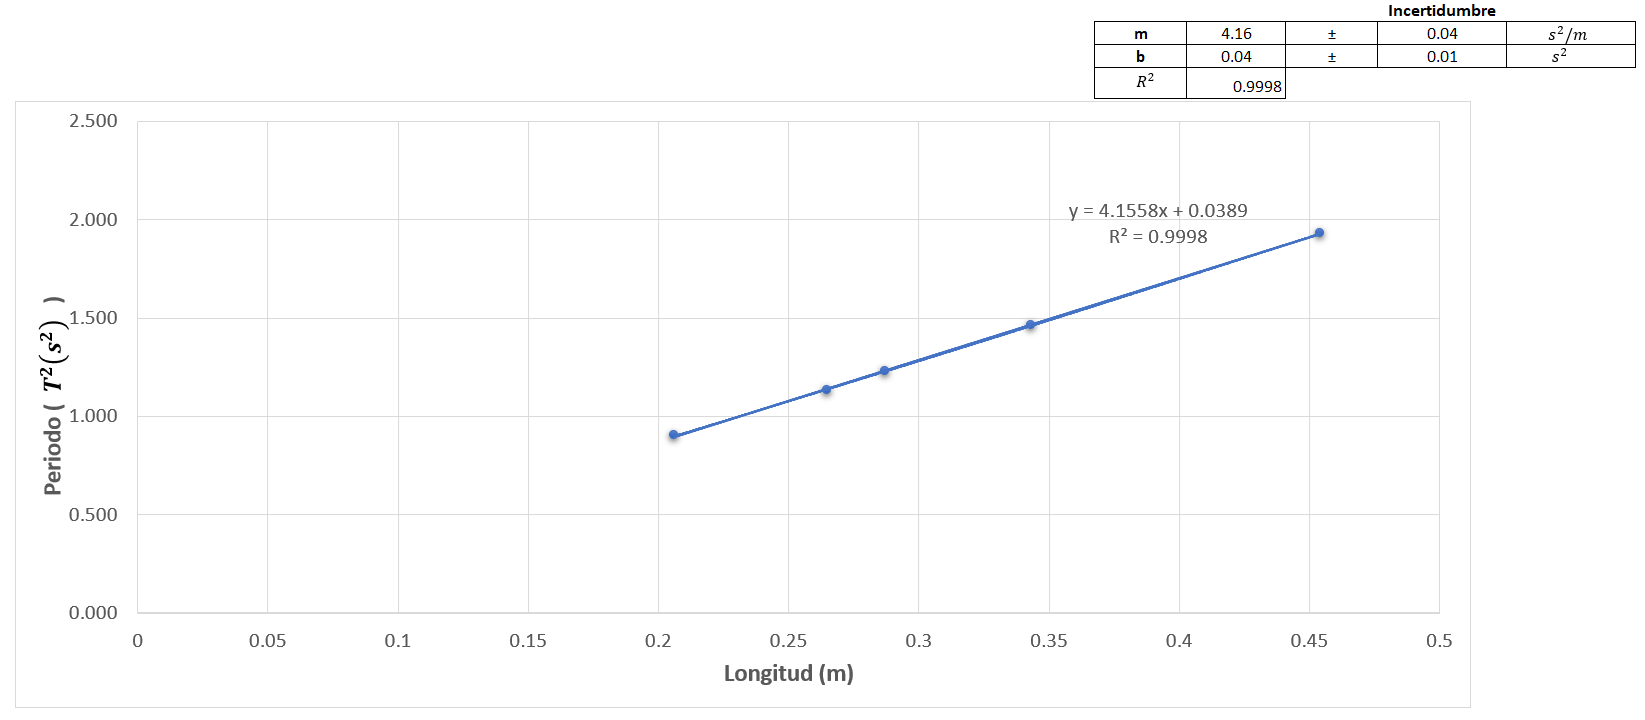
\includegraphics[scale=0.4]{imagenes-proyecto/grafico_t2_por_l.png}
	\captionsetup{justification=centering}
	\caption{Gráfica de $T^{2}$ vs $L$, a la vez con el ajuste linea y una tabla con la incertidumbre de la pendiente y el punto de corte o intercepto.}
	\label{Grafica T^2 VS L}
\end{figure}
\begin{multicols}{2}
En la Figura \ref{Grafica T^2 VS L}, se muestra la gráfica del cuadrado del periodo $(T^{2})$ por la longitud del péndulo (L), donde los puntos representan los datos experimentales, ahora se realiza el ajuste lineal para si conseguir la ecuación que relaciona estas dos variables, y realizando un análisis de datos podemos hallar la incertidumbre de la pendiente y el intercepto.
\begin{equation}
	y=4.1558 x +0.0389
	\label{ajuste1}
\end{equation}
Teniendo en cuenta ecuación \ref{10}, haremos que la ecuación sea directamente proporcional y así obtener la ecuación \ref{t2 lineal}, y lograr una dependencia lineal entre $(T^{2})$ y $(L)$

\begin{equation}
T^{2}=\frac{4 \pi^{2}}{g}L
\label{t2 lineal}
\end{equation}
 Ya teniendo la ecuación \ref{t2 lineal} igualamos con le ecuación \ref{ajuste1}, donde la pendiente será: 
 
\begin{equation}
 	m=\frac{4 \pi^{2}}{g}
 	\label{m_ecua}
\end{equation}
Luego, podemos observar que $(m)$ es la pendiente y lo tenemos de dato en la ecuación \ref{ajuste1}, y con esto podríamos determinar la aceleración de la gravedad experimental.
\begin{equation}
	g_{e}=\frac{4 \pi^{2}}{m}
	\label{g_ecua}
\end{equation}
\begin{equation}
	g_{e}=\frac{4 \pi^{2}}{4.1558} = 9.49 m/s^2
	\label{g_ecua_R}
\end{equation}
Entonces ya teniendo la gravedad experimental, podemos determinar la incertidumbre del módulo de la aceleración del gravedad $(\sigma_{g})$ realizando una propagación de incertidumbres, se obtiene que la expresión para hallar la incertidumbre del módulo de la aceleración de la gravedad es la ecuación \ref{g_incer_F}. Por lo tanto, usando la ecuación \ref{g_incer_F} y reemplazando el dato de la pendiente que lo tenemos en la ecuación \ref{ajuste1}, tal como también la incertidumbre del pendiente $(\sigma_{m})$ lo observamos en la Figura \ref{Grafica T^2 VS L}, por ende la ecuación será:

\begin{equation}
	\sigma_{g}=\frac{4\pi^2}{m^2}\sigma_{m}
	\label{g_incer_F}
\end{equation}
\begin{equation}
	\sigma_{g}=\frac{4\pi^{2}}{(4.1558)^2}(0.04) = 0.09m/s^2
	\label{g_incer_R}
\end{equation}
En consecuencia, obtendremos la siguiente:
\begin{equation}
	g_{e} = (9.49 \pm 0.09)  m/s^2
\end{equation}
A continuación, calcularemos el error porcentual de la gravedad con la ecuación \ref{grv_ecua_F}, teniendo como referencia el valor de la gravedad de la tierra según \cite{lange2012gravitacion} que será de $(9.81 m/s^2)$ y nuestro valor de la gravedad experimental, del resultado de la ecuación \ref{g_ecua_R}.
\begin{equation}
		Ep = \left | \frac{g{_{e}-g}}{g}\right |100\% 
		\label{grv_ecua_F}
\end{equation}
\begin{equation}
	Ep =\left |  \frac{9.49{_{e}-9.81}}{9.81} \right |100\% 
	\label{gr_ecua_for}
\end{equation}
\begin{equation}
	Ep = 3\%
	\label{gr_valor}
\end{equation}
\end{multicols}
%RESULTADOS 2
\begin{multicols}{2}

De la misma manera, se procede a realizar el segundo experimento, cabe resaltar que el péndulo debe estar a cierto ángulo, en esta ocasión repetiremos el ángulo tomado en el primer experimento, de 15°. Así mismo, para este experimento hemos elegido 5 masas distintas y una longitud de péndulo constante.\\
En la Tabla \ref{tabla de longitudes_2} se muestran los resultados experimentales del periodo y el masa. Así mismo se puede observar las incertidumbres, además se puede apreciar que hemos optado por usar 5 masas distintas con una longitud de péndulo constante.
\end{multicols}
% Colocar tablas y gráfica

% se escribe la tabla con los datos 
\begin{table}[ht]
	\centering
	\begin{tabular}{c c c c c c c c c}
		
		\hline\hline 
		%\vspace{2mm}
		
		%		Longitud $(m)$ & Periodo1 $(s)$ &Periodo2 $(s)$& Periodo3 $(s)$ & Periodo4$(s)$ &Periodo5 $(s)$& Promedio $(s)$& Incertidumbre $(s)$ \\ 
		Masa $(kg)$ & & & Periodos $(s)$& &  & Promedio $(s)$  & & Incertidumbre $(s)$  \\		
		\hline\hline	
		
		0.017&6.93&6.91&6.94&6.93&6.91&6.928&$\pm$& 0.006\\
		0.027&6.92&6.93&6.93&6.94&6.94&6.932&$\pm$& 0.004\\ 
		0.047&6.92&6.93&6.94&6.94&6.94&6.930&$\pm$& 0.004\\
		0.085&6.93&6.94&6.93&6.92&6.94&6.932&$\pm$& 0.004\\
		0.142&6.92&6.91&6.93&6.94&6.95&6.930&$\pm$& 0.007\\ [0.5ex]
		\hline	
	\end{tabular}
	\caption{Son los resultados logrados en nuestro segundo experimento, donde se visualiza las antecedentes experimentales de una variación de las masas, los tiempos de cinco oscilaciones o periodos $(s)$, el promedio $(s)$ y las incertidumbres del promedio. Teniendo en cuenta la incertidumbre de la longitud del péndulo de $ l= (0.4530\pm 0.0005m)$, así mismo la incertidumbre de la masa de $ \pm 0.001kg$}
	\label{tabla de longitudes_2}
	
\end{table}

\begin{table}[ht]
	\centering
	\begin{tabular}{c c c c}
		
		\hline\hline 
		%\vspace{2mm}
		
		Longitud $(m)$ & Periodo T  $(s)$& &  Incertidumbre de T $(s)$ \\ 
		
		\hline\hline	
		
		0.017&1.386&$\pm$&0.001\\
		0.027&1.386&$\pm$&0.001\\
		0.047&1.386&$\pm$&0.001\\
		0.085&1.386&$\pm$&0.001\\
		0.142&1.386&$\pm$&0.001\\ [0.5ex]
		\hline	
	\end{tabular}
	\caption{Son los resultados del segundo experimento, donde se tienen los datos procesados de los promedios $(s)$ en lo cual se obtiene un Periodo $T(s)$ y su incertidumbre.}
	\label{tabla de longitudes procesado_2}
\end{table}

\begin{figure}[H]
	\centering
	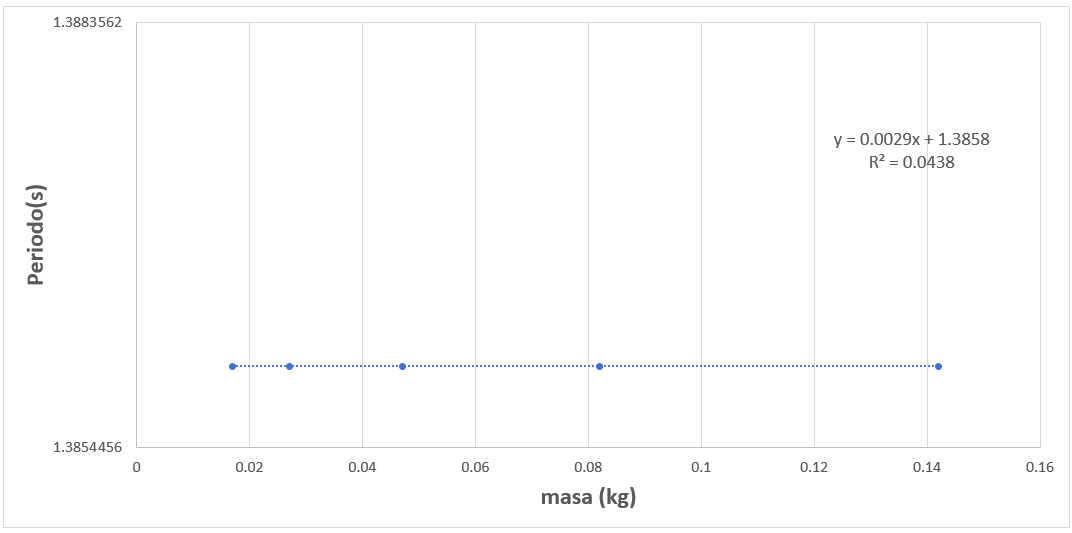
\includegraphics[scale=0.5]{imagenes-proyecto/grafica_Tvsm.png}
	\caption{Gráfica de $T$ vs $m$, a la vez con el ajuste linea.}
	\label{Grafica T VS m}
\end{figure}
En la Figura \ref{Grafica T VS m}, se puede comprobar que no existe una relación línea entre el periodo, puesto que los parámetros de ajuste notamos que la pendiente y el $R^2$ son muy pequeños y se observa un recta constante paralela al eje de la masa.\\

De acuerdo a los resultados obtenidos del Gráfico \ref{Grafica T^2 VS L} se comprueba el periodo al cuadrado si es directamente proporcional a la longitud, ya que la recta prácticamente se acerca al punto de origen y que nuestro factor de correlación es casi 1, además nuestra pendiente es positiva y nuestro intercepto es casi insignificante. Así mismo, analizando los datos logramos obtener la incertidumbre de la pendiente $(\pm 0.04 s^2/m)$ y del intercepto o punto de corte $(\pm 0.01 s^2)$, como se observa en la Figura \ref{Grafica T^2 VS L}.\\
Después, de hallar el módulo de la gravedad experimental obtenida de la ecuación \ref{g_ecua_R} $(9.49 m/s^2)$, podemos comparar con la gravedad de la tierra \cite{lange2012gravitacion} $(9.81 m/s^2)$ y con esto determinar su Error Porcentual usando la ecuación \ref{grv_ecua_F}, por lo que podemos indicar que el error es de $3\%$, este error se debe a al tiempo tomando por el cronómetro, es decir al iniciar y pausar el cronómetro, y también de la resistencia del aire en el ambiente donde se desarrolló el experimento.\\ 
Del Figura \ref{Grafica T VS m} realizando el ajuste lineal podemos indicar que la recta es paralela a eje de la masa y no pasa por el punto de origen, además observamos que la pendiente y el $R^2$ son muy pequeños, de modo que, no existe un relación lineal entre el periodo y la masa.

%%%%%%%%%%%%%%%%%%%%%%%%%%%%%%%
%%%%%%%%%%%%%%%%%%%%%%%%%%%%%%%
%Conclusiones	
\begin{multicols}{2}
	\section{Conclusiones}
	
En este experimento se ha alcanzado demostrar la relación que existe entre el periodo y la longitud en un péndulo simple, para el primer experimento se realizó el ajuste lineal de $T^2(s^2)vsL(m)$ en donde obtuvo la pendiente y el punto de corte o intercepto, y con esto se ha podido de determinar el módulo de la aceleración de la gravedad experimental, obteniendo un valor de $(9.49 m/s^2)$. \\
Además podemos observar que este valor muy cercano al valor real de la gravedad de la tierra $(9.81 m/s^2)$, debido a los pocos errores en la toma de valores en el experimento, además observamos que realizando el ajuste lineal obtenemos unos parámetros donde se muestra que el factor de correlación $(R^2)$ es muy cercano a 1 y el punto de corte es casi insignificante, como se observa en la Figura \ref{Grafica T^2 VS L}, y con esto se concluye que si existe tal relación, puesto que si variamos las longitudes los periodos van a ser diferentes.\\
Dado que nuestro valor de gravedad experimental es  $(9.49 m/s^2)$, podemos determinar la incertidumbre de la gravedad usando la ecuación \ref{g_incer_F}, por lo que hemos obtenido un valor de: $g_{e} = (9.49 \pm 0.09)  m/s^2$, entonces con esto precisar nuestro Error Porcentual $(E_{p})$, usando la fórmula \ref{grv_ecua_F}, podemos determinar que el error porcentual es de: $3\%$. Así mismo, este error de la gravedad experimental se debe a la resistencia del aire, los tiempos tomados con el cronómetro en el momento de pausar y también que nuestra masa realizaba un movimiento rotacional e hizo que nuestro movimiento traslacional se convirtiera en rotacional. Finamente, estos datos pueden mejorar teniendo un ambiente sin resistencia del aire y con mejores instrumentos de medición.\\
En el segundo experimento se ha demostrado que no existe una relación lineal entre el Periodo y la Masa, como se observa en la figura \ref{Grafica T VS m}, podemos concluir que se forma una lineal recta constante y paralela al eje de la masa, y no se acerca al punto de origen y también que pendiente es casi 0 y un factor de correlación es muy pequeño, además podemos observar en la tabla \ref{tabla de longitudes procesado_2} los valores de los Periodo $T(s)$ son prácticamente el mismo. Por ende, este experimento nos concluye que no existe un relación lineal entre el periodo y la masa.\\

\end{multicols}
	% Bibliografía
	\bibliographystyle{apalike}
	\bibliography{ref}
\end{document}